%
% File eacl2017.tex
%
%% Based on the style files for ACL-2016
%% Based on the style files for ACL-2015, with some improvements
%%  taken from the NAACL-2016 style
%% Based on the style files for ACL-2014, which were, in turn,
%% Based on the style files for ACL-2013, which were, in turn,
%% Based on the style files for ACL-2012, which were, in turn,
%% based on the style files for ACL-2011, which were, in turn, 
%% based on the style files for ACL-2010, which were, in turn, 
%% based on the style files for ACL-IJCNLP-2009, which were, in turn,
%% based on the style files for EACL-2009 and IJCNLP-2008...

%% Based on the style files for EACL 2006 by 
%%e.agirre@ehu.es or Sergi.Balari@uab.es
%% and that of ACL 08 by Joakim Nivre and Noah Smith

\documentclass[11pt]{article}
\usepackage{eacl2017}
\usepackage{times}
\usepackage{url}
\usepackage{csquotes}
\usepackage{amsmath}
\usepackage{latexsym}
\usepackage{comment} 
\usepackage{array}
\usepackage{multirow}
\usepackage{algorithm}
\usepackage{csquotes}
\usepackage{graphicx}
\usepackage{xspace}
\usepackage{subcaption}
\usepackage{color}
\usepackage{arydshln/arydshln}
\usepackage{amsfonts}
\usepackage{mathptmx} 
\usepackage{breqn}

\eaclfinalcopy % Uncomment this line for the final submission
%\def\eaclpaperid{***} %  Enter the acl Paper ID here

%\setlength\titlebox{5cm}
% You can expand the titlebox if you need extra space
% to show all the authors. Please do not make the titlebox
% smaller than 5cm (the original size); we will check this
% in the camera-ready version and ask you to change it back.

\newcommand\BibTeX{B{\sc ib}\TeX}

%\title{Using word sense as a filter to improve lexical substitution}
%\title{Word sense can improve lexical substitution rankings}
%\author{Anne Cocos$^*$ \and Marianna Apidianaki $^*,^\dag$ \and Chris Callison-Burch $^*$}\\

\title{Word Sense Filtering Improves Embedding-Based Lexical Substitution} % rankings}

\author{Anne Cocos$^{*}$, Marianna Apidianaki$^{*\dag}$ \and Chris Callison-Burch$^{*}$\\
$^{*}$ Computer and Information Science Department, University of Pennsylvania \\ 
$\dag$ LIMSI, CNRS, Universit\'e Paris-Saclay, 91403 Orsay \\
{\tt \{acocos,marapi,ccb\}@seas.upenn.edu} \\}


%\author[1]{Anne Cocos}
%\author[1]{Marianna Apidianaki}
%\affil[1]{Computer and Information Science Department, University of Pennsylvania}
%\affil[$\dag$] {LIMSI, CNRS, Universitee Paris-Saclay, 91~403 Orsay}\\

%\renewcommand\Authands{ and }
\date{}

\begin{document}
\maketitle
\begin{abstract}

The role of word sense induction and disambiguation in lexical substitution has been questioned due to the high performance of vector space models which propose good substitutes without accounting for sense. We show that a filtering mechanism based on a sense inventory optimized for substitutability can improve the results of these models. Our sense inventory is constructed using a clustering method which generates paraphrase clusters that are congruent with lexical substitution annotations in a development set. The results show that lexical substitution can still benefit from senses which can improve the output of vector space ranking models.

\end{abstract}

\section{Introduction}

Word senses have always been difficult to define and pin down \cite{kilgarriff1997don,ErketalCL2013}, and recent successes of embedding-based models in various semantic tasks are further challenging people's belief in them. Why bother to identify senses if even humans do not manage to come to an agreement on their nature and number, and if simple word-embedding models yield good results without needing any sense representations? 
%can yield similar or better results in tasks as disambiguation approaches? 

Word-based models are   successful in various semantic tasks even though they conflate the different meanings of words into a single representation. Departing from the assumption that capturing polysemy %sense distinctions 
could further improve their performance, several works have focused on creating sense-specific embeddings. % either by clustering 
%to developping multiple embeddings per word type is by %pre-clustering the contexts of each token into a fixed number of senses for each word, and then relabelling each word token with the clustered sense before learning embeddings \cite{reisinger-mooney:2010:NAACLHLT,huang-EtAl:2012:ACL20122}. 
A common approach is to cluster the contexts in which the words appear in a corpus into senses %into a fixed number of clusters/senses %of each token of a word in a corpus into a fixed number of senses, 
and relabel each word token with the clustered sense before embedding learning  \cite{reisinger-mooney:2010:NAACLHLT,huang-EtAl:2012:ACL20122}. %\newcite{Liu:2015:TWE:2886521.2886657} learn sense specific embeddings using %by combining neural frameworks with LDA topic models.
\newcite{iacobacci-pilehvar-navigli:2015:ACL-IJCNLP} disambiguate the words in a corpus using a state-of-the-art WSD system and then produce continuous representations of word senses based on the distributional information obtained from the annotated corpus. %before learning the embeddings. 
%Similarly, \newcite{iacobacci-pilehvar-navigli:2015:ACL-IJCNLP} first disambiguate the instances of words in a corpus using a state-of-the-art WSD system and then process the disambiguated text with the word2vec toolkit \cite{Mikolovetal2013} to produce continuous represenations of word senses based on the distributional information obtained from the annotated corpus. 
Moving from word to sense embeddings generally improves their performance in word and relational similarity tasks but is not beneficial in all settings. 
\newcite{li-jurafsky:2015:EMNLP} show that although multi-sense embeddings give improved performance in tasks such as semantic similarity, semantic relation identification and part-of-speech tagging, they don't help in others, like sentiment analysis and named entity extraction \cite{li-jurafsky:2015:EMNLP}. %Apart from learning sense-specific representations, 

We show how a sense inventory optimized for \textit{substitutability} can improve the rankings provided by two sense agnostic vector-based lexical substitution models. 
%two lexical substitution models. We show how senses optimized for substitutability %induced from paraphrase data can help vector- and embedding-based lexical substitution models. 
Lexical substitution is a task where systems are required to predict substitutes  for target word instances which preserve their meaning in specific contexts \cite{mccarthy-navigli:07}. We carry out experiments with a syntactic vector-space model \cite{apidianaki:2016:EMNLP2016} and a word-embedding model  for lexical substitution \cite{melamud-levy-dagan:2015:VSM-NLP}. %Contrary to \newcite{faruqui-EtAl:2015:NAACL-HLT} who used semantic lexicons %such as WordNet, FrameNet and the Paraphrase Database 
%to refine vector representations, %\footnote{In this work, relational information from WordNet, FrameNet and the Paraphrase Database served to encourage linked words to have similar vector representations.} 
Instead of using the senses to refine the vector representations as in \cite{faruqui-EtAl:2015:NAACL-HLT}, we rather use them to improve the lexical substitution rankings proposed by the models. We show that senses can improve the performance of vector-space models in lexical substitution tasks.
% in a task. 
% The old debate around word senses, their nature and utility in applications has recently been enriched with considerations on their abandomnent in favor of simpler word-based representations. 
%Simple word embedding %models have been shown to efficiently perform complex semantic processing tasks without need for semantic lexicons and disambiguation techniques. 
%Given the  difficulty to identify senses (Kilgarriff) and the multiplicity of possible representations, why bother with them if word-based models can perform the same tasks as efficiently? 
%However, in spite of the increasing popularity of distributed representations, several works show that their quality can be improved using senses and paraphrases from semantic lexicons. 

%In this paper, we explore the performance of vector-space and embedding models on a lexical substitution task, with and without using senses. Our models come from 


\section{A sense inventory for substitution}

\subsection{Paraphrase substitutability}

The candidate substitutes used by the ranking models come from the Paraphrase Database (PPDB) XXL package \cite{ganitkevitch-EtAl:2013:NAACL}.\footnote{{\sc ppdb} paraphrases come into packages of different sizes (going from {\sc s} to {\sc xxxl}): small packages contain high-precision paraphrases while larger ones have high coverage.} Paraphrase relations in the PPDB are defined between words and phrases which might carry different senses. \newcite{cocos-callisonburch:2016:N16-1} used a spectral clustering algorithm to cluster PPDB XXL into senses, but % and found that using distributional similarity to weight the edges in the input graph led to clusters that generally captured word sense. 
the clusters contain noisy paraphrases and paraphrases linked by different types of relations (e.g. hypernyms, antonyms) which are not always substitutable. We use a slightly modified version of their method to cluster paraphrases where both the number of clusters/senses and their contents are optimized for substitutability. % this time optimizing for substitutability.  %We create a new clustering where both the number of clusters/senses and their contents are optimized for substitutability.

%Each word pair also has a real-valued score (PPDB2.0 Score) indicating the strength of the paraphrase relationship \cite{pavlick2015ppdb}. Given a target word \textit{t}, we call its set of PPDB paraphrases $P(t)$. Note that $P(t)$ excludes $t$ itself.

%a lot of noisy paraphrases. Furthermore, as this inventory was built from the XXL package, paraphrases are linked by various types of relations and are often not substitutable in context. In this work, we use paraphrase clusters optimized for substitutability. Using a paraphrase threshold tuned on the data, noisy paraphrases are filtered out. We also define a measure of substitutability and choose the optimal clustering solution respective to this measure. 

\subsection{A measure of substitutability}
\label{nmi} 

We define a substitutability metric that quantifies the extent to which a sense inventory aligns with human-generated lexical substitution annotations. We then cluster PPDB paraphrases using the substitutability metric to optimize the sense clusters for substitutability. 
%The resulting sense clusters have both wide vocabulary coverage and high substitutability. Finally we show, via an oracle experiment, that it is possible to use the resulting sense clusters to filter LexSub rankings generated by embedding-based models in order to boost the ranking of the best substitution candidates. 
 %{\sc ppdb} paraphrases come into packages of different sizes (going from {\sc s} to {\sc xxxl}): smaller packages contain high-precision paraphrases while larger ones aim for high coverage. 
%PPDB contains milions of paraphrases and has higher coverage than other semantic resources (e.g. WordNet). We use one of the biggest PPDB packages, the XXL one, and collect the paraphrases available for a set of 327 target words extracted from the ``Concepts in Context" (CoInCo) lexical substitution dataset which comprises manually annotated with single and multi-word substitutes \cite{kremer-EtAl:2014:EACL}. Paraphrase relations in the PPDB are between words. A clustering of the English paraphrases into senses exists \cite{cocos-callisonburch:2016:N16-1} but the clusters contain a lot of noisy paraphrases. Furthermore, as this inventory was built from the XXL package, paraphrases are linked by various types of relations and are often not substitutable in context. In this work, we use paraphrase clusters optimized for substitutability. Using a paraphrase threshold tuned on the data, noisy paraphrases are filtered out. We also define a measure of substitutability and choose the optimal clustering solution respective to this measure. 

Given a sense inventory $C$, we can define the senses of a target word $t$ as a set of sense clusters, $C(t) = \{c_1, c_2, \dots c_k\}$, where each cluster contains words corresponding to a single sense of $t$. Intuitively, if a sense inventory corresponds with substitutability, then each sense cluster $c_i$ should have two qualities: first, words within $c_i$ should be interchangeable with $t$ in the same set of contexts; and second, $c_i$ should not be missing any words that are interchangeable in those same contexts. We therefore operationalize the definition of substitutability as follows. 

We begin with a %(human-annotated) 
lexical substitution dataset, the ``Concepts in Context" (CoInCo) corpus \cite{kremer-EtAl:2014:EACL}, consisting of sentences where content words have been manually annotated with substitutes.\footnote{CoInCo contains over 15K sentences corresponding to nearly 4K unique content words.} 
%target words, a set of sentences for each target word, and a set of annotated substitutes for each sentence (Table \ref{tab:lexsub}). 
We then use normalized mutual information (NMI) \cite{strehl2002cluster} to quantify the level of agreement between the sense clusters and human-suggested substitutes. NMI is an information theoretic measure of cluster quality. Given two clusterings $U$ and $V$ over a set of items, it measures how much each clustering reduces uncertainty about the other \cite{vinh2009information} in terms of their mutual information $I(U,V)$ and entropies $H(U), H(V)$:

\begin{table}[t]
%	\centering
	\small
	\begin{tabular}{p{0.38\columnwidth} p{0.52\columnwidth}}
		\hline
		Sentence & Annotated Substitutes (Count) \\ \hline \hline
		In this world, one's \textbf{word} is a promise. & vow (1), utterance (1), tongue (1), speech (1) \\ \hline
		Silverplate: code \textbf{word} for the historic mission that would end World War II. & phrase (3), term (2), verbiage(1), utterance (1), signal (1), name (1), dictate (1), designation (1), decree (1) \\ \hline
		I think she only heard the last \textbf{words} of my speech. & bit (3), verbiage (2), part (2), vocabulary (1), terminology (1), syllable (1), phrasing (1), phrase (1), patter (1), expression (1), babble (1), anecdote (1) \\
	\end{tabular}
	\caption{Example annotated sentences for the target word \textit{word.N} from the CoInCo lexical substitution dataset. Numbers after each word indicate the number of annotators who made that suggestion.}
	\label{tab:lexsub}
\end{table}

%\[H(U) = - \sum_{i=1}^R{\frac{a_i}{N}\log \frac{a_i}{N}}\]
%
%\[H(V) = - \sum_{j=1}^C{\frac{b_j}{N}\log \frac{b_j}{N}}\]
%
%\[I(U,V) = \sum_{i=1}^R\sum{j=1}^C \frac{n_{ij}}{N} \log \frac{n_{ij}/N}{a_ib_j/N^2}\]

\[NMI(U,V) = \frac{I(U,V)}{\sqrt{H(U)H(V)}}\]

\noindent To calculate the NMI between a sense inventory for target word \textit{t} and its set of annotated substitutes, we first define the substitutes as a clustering, $B_t = \{b_1, b_2, \dots b_n\}$, where $b_i$ denotes the set of suggested substitutes for each of $n$ sentences. Table \ref{tab:lexsub}, for example, gives the clustered substitutes for $n=3$ sentences for target word $t=\text{word.N}$, where $b_1 = \{\text{vow, utterance, tongue, speech}\}$. We then define the substitutability of the sense inventory, $C_t$, with respect to the annotated substitutes, $B_t$, as $NMI(C_t, B_t)$.\footnote{In calculating NMI, we ignore words that do not appear in both $C_t$ and $B_t$.} Given many target words, we can further aggregate the substitutability of sense inventory $C$ over the set of targets $T$ in $B$ into a single substitutability score:
\[substitutability_B(C) = \sum_{t \in T} \frac{NMI(C_t, B_t)}{|T|}\]

\subsection{Optimizing for Substitutability}
\label{optim}

Having defined a substitutability score, we now automatically generate word sense clusters from the Paraphrase Database that maximize it. The idea is to use the substitutability score to choose the best number of senses for each target word which will be the number of output clusters (\textit{k}) needed by our spectral clustering algorithm. 
%\subsection{Data}\label{section:data}
%\label{dev}

In order to perform this optimization, we first divide the CoInCo dataset into development and test sets as follows. We find all target words in the CoInCo dataset that have at least 10 sentences. For each of the 327 resulting targets, we randomly divide the corresponding sentences into 60\% development instances and 40\% test instances. The resulting development and test sets have 4061 and 2091 sentences respectively. We cluster the 327 target words in the resulting subset of CoInCo, performing all optimization using the development portion, and running evaluation on the test portion.

\begin{comment}
\subsection{Spectral clustering method}

PPDB contains word pairs that have been found to be paraphrases using the pivot method \cite{bannard2005paraphrasing}. Each word pair also has a real-valued score (PPDB2.0 Score) indicating the strength of the paraphrase relationship \cite{pavlick2015ppdb}. Given a target word \textit{t}, we call its set of PPDB paraphrases $P(t)$. Note that $P(t)$ excludes $t$ itself.

\newcite{cocos-callisonburch:2016:N16-1} used a spectral clustering algorithm to cluster PPDB XXL. They found that using distributional similarity to weight the edges in the input graph led to clusters that generally captured word sense. We use a slightly modified version of their method to cluster PPDB XXL paraphrases, this time optimizing for substitutability. 
\end{comment}

\subsection{Spectral clustering method}
\subsubsection{Constructing the Affinity Matrix}

The spectral clustering algorithm \cite{yu2003multiclass} takes as input an affinity matrix $A \in \mathbb{R}^{n\times n}$ encoding $n$ items to be clustered, and an integer $k$. It generates $k$ non-overlapping clusters of the $n$ items. Each entry $a_{ij}$ in the affinity matrix denotes a similarity measurement between items $i$ and $j$. Entries in $A$ must be nonnegative and symmetric. The affinity matrix can also be thought of as describing a graph, where the $n$ rows and columns correspond to nodes, and each entry $a_{ij}$ gives the weight of an edge between nodes $i$ and $j$. Because the matrix must be symmetric, the graph is undirected.

Given a target word \textit{t}, we call its set of PPDB paraphrases $P(t)$. Note that $P(t)$ excludes $t$ itself. In our most basic clustering method, we cluster paraphrases for target $t$ as follows. Given the length-$n$ set of $t$'s paraphrases, $P(t)$, we construct the $n \times n$ affinity matrix $A$ where each shared-index row and column corresponds to some word $p \in P(t)$. We set entries equal to the cosine similarity between the applicable words' embeddings, plus one: $a_{ij} = cos(v_i,v_j) + 1$ (to enforce non-negative similarities). For our implementation we use 300-dimensional part-of-speech-specific word embeddings $v_i$ generated using the gensim word2vec package \cite{mikolov2013distributed,mikolov2013efficient,ismu:884893} \footnote{The \texttt{word2vec} parameters we use are a context window of size 3, learning rate \textit{alpha} from 0.025 to 0.0001, minimum word count 100, sampling parameter $1e^{-4}$, 10 negative samples per target word, and 5 training epochs.}. A diagram showing a set of paraphrases and their corresponding basic affinity matrix is given in figures \ref{fig:ppgraph} and \ref{fig:ppmatall}.

In order to aid further discussion, we point out that the affinity matrix used for the basic clustering method encodes a fully-connected graph $G = \{P(t), E_{PP}^{ALL}\}$ with paraphrases $P(t)$ as nodes, and edges between every pair of words, $E_{PP}^{ALL} = P(t) \times P(t)$. As for all variations on the clustering method, the matrix entries correspond to distributional similarity.

\begin{figure*}
	\begin{subfigure}[t]{0.25\textwidth}
		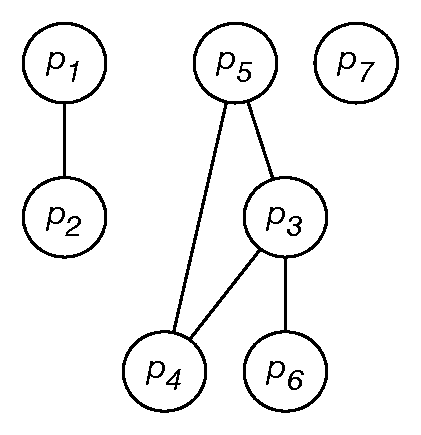
\includegraphics[width=\textwidth]{images/pp_graph.pdf}
		\caption{PPDB graph with $n=7$ paraphrases $P(t)$ to be clustered.}
		\label{fig:ppgraph}
	\end{subfigure}
	\hfill%
	\begin{subfigure}[t]{0.36\textwidth}
		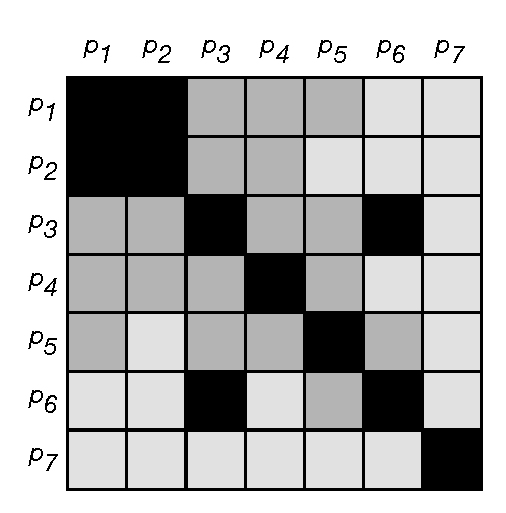
\includegraphics[width=\textwidth]{images/pp_mat_all.pdf}
		\caption{\textit{Unmasked} affinity matrix for input to basic clustering algorithm, for paraphrases in Fig \ref{fig:ppgraph}. This matrix encodes a fully-connected graph $G = \{P(t), E_{PP}^{ALL}\}$.}
		\label{fig:ppmatall}
	\end{subfigure}
	\hfill%
	\begin{subfigure}[t]{0.36\textwidth}
		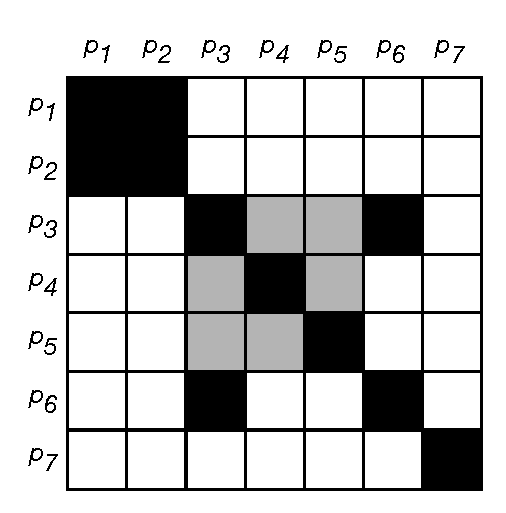
\includegraphics[width=\textwidth]{images/pp_mat_mask.pdf}
		\caption{\textit{Masked} affinity matrix for input to clustering algorithm, enforcing the paraphrase links from the graph in Fig \ref{fig:ppgraph}, $G = \{P(t), E_{PP}^{MASK}\}$.}
		\label{fig:ppmatmask}
	\end{subfigure}
	\caption{Unclustered PPDB graph and its corresponding affinity matrices for input to the basic (\ref{fig:ppmatall}) and masked (\ref{fig:ppmatmask}) clustering algorithms. Cell shading corresponds to the distributional similarity score between words, with darker colors representing higher measurements. }
\end{figure*}

\subsubsection{Masking}

The affinity matrix described above ignores the graph structure inherent in PPDB, where edges connect only words that are paraphrases of one another. We experiment with enforcing the PPDB structure in the affinity matrix through masking. 

In the masked affinity matrix, we set each entry $a_{ij}$ for which $i$ and $j$ are \textit{not} paraphrases in PPDB to zero. The masked affinity matrix encodes the graph $G = \{P(t), E_{PP}^{MASK}\}$ with edges connecting only pairs of words that are in PPDB, $E_{PP}^{MASK} = \{(p_i, p_j) \mid p_i \in P(p_j)\}$. Figure \ref{fig:ppmatmask} shows the masked affinity matrix corresponding to the PPDB structure in Figure \ref{fig:ppgraph}.

\subsubsection{Optimizing \textit{k}}
\label{optimk}

Because spectral clustering requires the number of output clusters, $k$, to be specified as input, for each target word we run the clustering algorithm for a range of $k$ between 1 and the minimum of ($n$,  20). We then choose the \textit{k} that maximizes the NMI of the resulting clusters with the human-annotated substitutes for that target from the CoInCo develpment dataset, as explained in Sections \ref{nmi} and \ref{optim}.

\subsection{Method variations}

In addition to using the substitutability score to choose the best number of senses for each target word, we also experiment with %three %using word embeddings that have been retrofitted to LexSub annotation data, 
two variations on the basic spectral clustering method to increase the score further: filtering by a paraphrase confidence score and co-clustering with WordNet \cite{fellbaum98wordnet}. 


\subsubsection{PPDB Score Thresholding}

%PPDB contains word pairs that have been found to be paraphrases using the pivot method \cite{bannard2005paraphrasing}. 
Each paraphrase pair in the PPDB is associated with a set of scores indicating the strength of the paraphrase relationship. The recently added PPDB2.0 Score \cite{pavlick-EtAl:2015:ACL-IJCNLP3} was calculated using a 
%The good performance of Ppdb2 is due to the use of a 
supervised scoring model trained on human judgments of paraphrase quality.\footnote{The human judgments were used to fit a regression to the features available in {\sc ppdb} 1.0 plus numerous new features including cosine word embedding similarity, lexical overlap features, WordNet features and distributional similarity features.}
%\footnote{The features used for computing the paraphrase ranking in {\sc ppdb} 2.0 are described in detail in Pavlick et al. \shortcite{pavlick-EtAl:2015:ACL-IJCNLP3}.} 
%real-valued score (PPDB2.0 Score) indicating the strength of the paraphrase relationship \cite{pavlick2015ppdb}. 
\newcite{apidianaki:2016:EMNLP2016} showed that the PPDB2.0 Score itself is a good metric for ranking substitution candidates in context, outperforming some vector space models when the number of candidates is high. With this in mind, we experimented with using a PPDB2.0 Score threshold to discard noisy PPDB XXL paraphrases prior to sense clustering. Our objective was to begin the clustering process with a \textit{clean} set of paraphrases for each target word, eliminating erroneous paraphrases that might pollute the substitutable sense clusters. We implemented PPDB score thresholds in a range from 0 to 2.5.

\begin{comment}
\subsubsection{Retrofitted Vectors}

Our overall objective in clustering was to generate clusters that are fully substitutable. But the distributional similarity measure we used as input to the clustering algorithm is known to confuse \textit{semantic similarity} and \textit{conceptual association} \cite{hill2016simlex}, producing high similarity measurements between dissimilar words like antonyms \cite{mohammad2008computing,mrkvsic2016counter}. We sought a similarity metric that better captures substitutability. Therefore we also experimented with retrofitting the word embeddings to a semantic lexicon created from LexSub annotation data prior to clustering \cite{faruqui2014retrofitting}.

The retrofitting method of \newcite{faruqui2014retrofitting} refines vector space representations of words using relational information from semantic lexicons (i.e. sets of similar words). Given any set of pre-trained word embeddings, it encourages words appearing within a lexicon group to move closer in vector space. We ran the retrofitting tool on our part-of-speech-specific word embeddings, using human-annotated substitutes from the TWSI\footnote{URL} and CoInCo (development portion) datasets as the input lexicon. The result is a set of word embeddings for which words that have been deemed 'substitutable' by human annotators are closer together. We then experiment with using the substitutability-retrofitted word embeddings (in place of the generic word embeddings) in our clustering model.
\end{comment}

\begin{figure*}[th]
	\begin{subfigure}[t]{0.25\textwidth}
		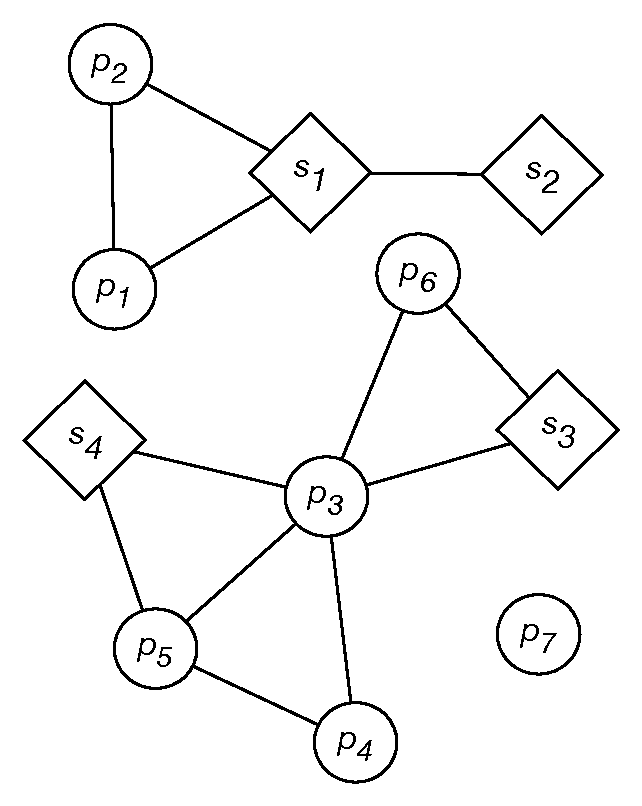
\includegraphics[width=\textwidth]{images/pp_syn_graph.pdf}
		\caption{Graph showing $n=7$ PPDB paraphrases $P(t)$ and $m=4$ WordNet synsets $S^+(t)$ to be clustered.}
		\label{fig:ppsyngraph}
	\end{subfigure}
	\hfill%
	\begin{subfigure}[t]{0.36\textwidth}
		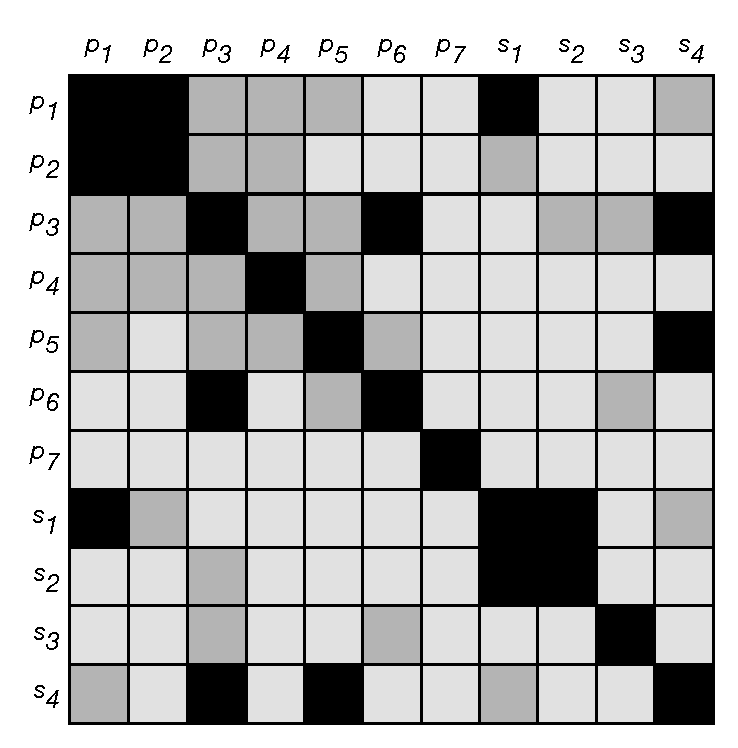
\includegraphics[width=\textwidth]{images/pp_syn_mat_all.pdf}
		\caption{\textit{Unmasked} affinity matrix for input to basic clustering algorithm, for paraphrases and synsets in Fig \ref{fig:ppsyngraph}. This matrix encodes a fully-connected graph $G = \{P(t) \cup S^+(t), E_{PP}^{ALL} \cup E_{PS}^{ALL} \cup E_{SS}^{ALL} \}$.}
		\label{fig:ppsynmatall}
	\end{subfigure}
	\hfill%
	\begin{subfigure}[t]{0.36\textwidth}
		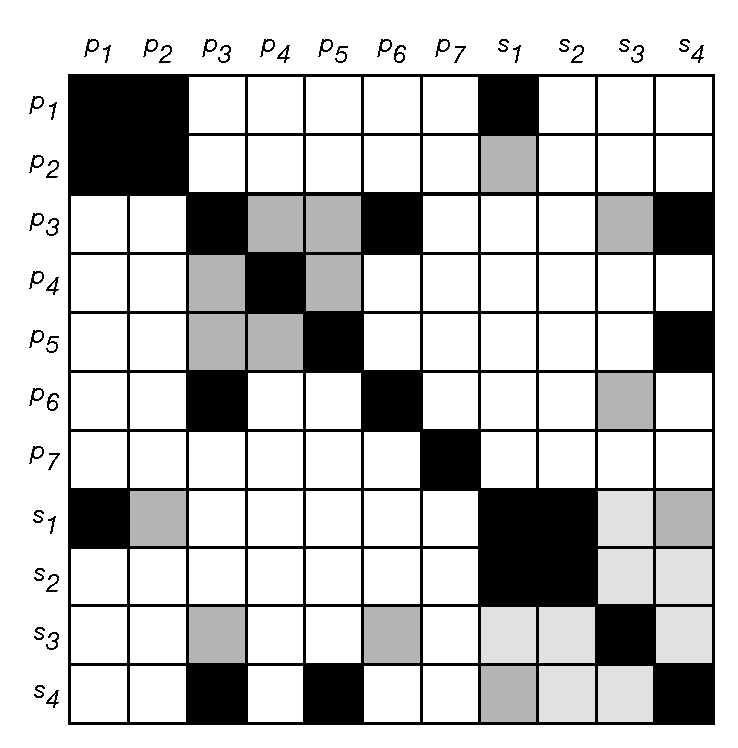
\includegraphics[width=\textwidth]{images/pp_syn_mat_mask.pdf}
		\caption{Affinity matrix for input to clustering algorithm, enforcing the paraphrase-paraphrase ($E_{PP}^{MASK}$) and paraphrase-synset ($E_{PS}^{MASK}$) links from the graph in \ref{fig:ppsyngraph}, but allowing all synset-synset links ($E_{PP}^{ALL}$). }
		\label{fig:ppsynmatmask}
	\end{subfigure}
	\caption{Paraphrase/synset graph for input to the co-clustering model, and its corresponding affinity matrices for the basic (\ref{fig:ppsynmatall}) and masked (\ref{fig:ppsynmatmask}) clustering algorithms. Cell shading corresponds to the distributional similarity score between words/synsets. }
	\label{fig:cocluster}
\end{figure*}


\subsubsection{Co-Clustering with WordNet}

PPDB is large and inherently noisy. WordNet %, which proved to be the most 'substitutable' sense inventory in earlier experiments (Table \ref{tab:nmi}), 
has smaller coverage but well-defined semantic structure in the form of synsets and relations. We sought a way to marry the high coverage of PPDB with the clean structure of WordNet by co-clustering the two resources, in hopes of creating a sense inventory that is both highly-substitutable, and high-coverage. %Creating a mapping between the two resources will help to structure the PPDB and increase the coverage of WordNet. 

The basic unit in WordNet is the \textit{synset}, a set of lemmas sharing the same meaning. WordNet also connects synsets via relations, such as hypernymy, hyponymy, entailment, and `similar-to'. We denote as $L(s)$ the set of lemmas associated with synset $s$. We denote as $R(s)$ the set of synsets that are related to synset $s$ with a hypernym, hyponym, entailment, or similar-to relationship. Finally, we denote as $S(t)$ the set of synsets to which a word $t$ belongs. We denote as $S^+(t)$ the set of $t$'s synsets, plus all synsets to which they are related; $S^+(t) = S(t) \cup \bigcup_{s^\prime \in S(t)} S(s^\prime)$. In other words, $S^+(t)$ includes all synsets to which $t$ is connected by a path of length at most 2 via one of the relations encoded in $R(s)$.

For co-clustering, we generate the affinity matrix for a graph with $m+n$ nodes corresponding to the $n$ words in $P(t)$ and the $m$ synsets in $S^+(t)$, and edges between every pair of nodes. Because the edge weights are cosine similarity between vector embeddings, we need a way to construct an embedding for each synset in $S^+(t)$.\footnote{We don't use the NASARI embeddings \cite{camachocollados-pilehvar-navigli:2015:NAACL-HLT} because these are available only for nouns.} We therefore generate compositional embeddings for each synset $s$ that are equal to the weighted average of the embeddings for the lemmas $l \in L(s)$, where the weights are the PPDB2.0 score between $t$ and $l$:

\[v_s = \frac{\sum_{l \in L(s)} PPDB2.0Score(t, l) \times v_l}{\sum_{l \in L(s)} PPDB2.0Score(t, l)}\]

\noindent The unmasked affinity matrix used for input to the co-clustering method, then, encodes the graph $G = \{P(t) \cup S^+(t), E_{PP}^{ALL} \cup E_{PS}^{ALL} \cup E_{SS}^{ALL} \}$, where $E_{PS}^{ALL}$ contains edges between every paraphrase and synset, and $E_{SS}^{ALL}$ contains edges between every pair of synsets.

We also define masked versions of the co-clustering affinity matrix. Just as we defined masking for $E_{PP}$, we separately define masking for paraphrase-synset links $E_{PS}$ and synset-synset links $E_{SS}$. When applying the clustering algorithm, it is possible to elect to use the masked version for any or all of $E_{PP}$, $E_{PS}$, and $E_{SS}$. In our experiments we try all combinations.

For the synset-synset links, we define the masked version $E_{SS}^{MASK}$ as including only nonzero edge weights where a hypernym, hyponym, entailment, or similar-to relationship connects two synsets: $E_{SS}^{MASK} = \{(s_u, s_v) \mid s_u \in R(s_v) \text{ or } s_v \in R(s_u)\}$. For the paraphrase-synset links, we define the masked version $E_{PS}^{MASK}$ to include only nonzero edge weights where the paraphrase \textit{is} a lemma in the synset, or \textit{is a paraphrase of} a lemma in the synset (excluding the target word): $E_{PS}^{MASK} = \{(p_i, s_u) \mid p_i \in L(s_u) \text{ or } |(P(p_i)-t) \cap L(s_u)| > 0 \}$. We need to exclude the target word when calculating the overlap because otherwise all words in $P(t)$ would connect to all synsets in $S(t)$. Figure \ref{fig:cocluster} depicts the graph, unnmasked, and masked affinity matrices for the co-clustering method. 


\section{Filtering Substitutes}

\subsection{A WSD oracle}

We now question whether it is possible to improve the rankings of current state-of-the-art lexical substitution systems by using the optimized sense inventory as a filter. Our general approach is to take a set of ranked substitutes generated by a vector-based model. Then, we see whether filtering the ranked substitutes to bring words belonging to the correct sense of the target to the top of the rankings would improve the overall ranking results. 

Assuming that we have a WSD oracle that is able to choose the most appropriate sense for a target word in context, this corresponds to nominating substitutes from the applicable sense cluster and pulling them up in the list of ranked substitutes output by the state-of-the-art lexical substitution ranking system. 
%, and ranking them according to the state-of-the-art lexical substitution ranking system. 
If sense filtering successfully improves the quality of ranked substitutes, we can say that the sense inventory captures substitutability well. 

%\subsection{Data}

We use the test portion of the CoInCo subset defined in Section \ref{optim} to evaluate the extent to which our optimized sense inventories improve lexical substitution rankings. Recall that the test portion consists of 2091 annotated sentences for 327 target words.


\subsection{Ranking Models}

Our approach requires a set of rankings produced by a high-quality lexical substitution model to start. We generate substitution rankings for each target/sentence pair in the test set using a syntactic vector-space model \cite{thater-furstenau-pinkal:2011:IJCNLP-2011,apidianaki:2016:EMNLP2016} and a state-of-the-art model based on word embeddings \cite{melamud-levy-dagan:2015:VSM-NLP}. 

The syntactic vector space model of \newcite{apidianaki:2016:EMNLP2016} (Syn.VSM) demonstrated an ability to correctly choose appropriate PPDB paraphrases for a target word in context. The vector features correspond to syntactic dependency triples extracted from the English Gigaword corpus \footnote{\url{http://catalog.ldc.upenn.edu/LDC2003T05}} analysed with Stanford dependencies \cite{mcdm:06}. Syn.VSM produces a score for each (target, sentence, substitute) tuple based on the cosine similarity of the substitute's basic vector with the target's contextualized vector \cite{thater-furstenau-pinkal:2011:IJCNLP-2011}. The contextualised vector is derived from the basic meaning vector of the target word by reinforcing its dimensions that are licensed by the context of the specific instance under consideration. More specifically, the contextualised vector of a target is obtained through vector addition and contains information about the target's direct syntactic dependents. %its context words in the sentence.

The second set of rankings comes from the AddCos model of \newcite{melamud-levy-dagan:2015:VSM-NLP}. AddCos quantifies the fit of substitute word $s$ for target word $t$ in context $C$ by measuring the semantic similarity of the substitute to the target, and the similarity of the substitute to the context:

\begin{dmath}
	AddCos(s,t,W) = \frac{|W| \cdot cos(s,t) + \sum_{w \in W} cos(s,w)}{2 \cdot |W|}
\end{dmath}
	
\noindent The vectors $s$ and $t$ are word embeddings of the substitute and target generated by the \textit{skip-gram with negative sampling} model \cite{mikolov2013distributed,mikolov2013efficient}. The context $W$ is the set of words appearing within a fixed-width window of the target $t$ in a sentence (we use a window (cwin) of 1), and the embeddings $c$ are context embeddings generated by \textit{skip-gram}. In our implementation, we train 300-dimensional word and context embeddings over the 4B words in the Annotated Gigaword (AGiga) corpus \cite{napoles2012annotated} using the gensim word2vec package \cite{mikolov2013distributed,mikolov2013efficient,ismu:884893}. \footnote{The \texttt{word2vec} training parameters we use are a context window of size 3, learning rate \textit{alpha} from 0.025 to 0.0001, minimum word count 100, sampling parameter $1e^{-4}$, 10 negative samples per target word, and 5 training epochs.}

\subsection{Baselines}
%\section{Evaluating Substitutability}

%We evaluate three baseline sense inventories. 

We compare the extent to which our optimized sense inventories improve lexical substitution rankings to the results of two baseline sense inventories.

\begin{itemize}
\item\textbf{WordNet+}: a sense inventory formed from WordNet 3.0. For each CoInCo target word that appears in WordNet, we take its sense clusters to be its synsets, plus lemmas belonging to hypernyms and hyponyms of each synset. 
\item\textbf{PPDBClus}: a much larger, abeit noisier, sense inventory obtained by automatically clustering words in the PPDB XXL package. To obtain this sense inventory we clustered paraphrases for all targets in the CoInCo dataset using the method outlined in \newcite{cocos-callisonburch:2016:N16-1}, with PPDB2.0 Score serving as the similarity metric.
%\item\textbf{TWSI}: the Turk Bootstrap Word Sense Inventory v2 (TWSI) \cite{Biemann:2013} is a crowdsourced sense inventory constructed specifically for substitutability. 
\end{itemize}

\begin{table}[t]
	\centering
	\begin{tabular}{p{1.7cm} *{2}{p{1.6cm}} p{1.3cm}}
		\hline
		Sense  Inventory & Avg \# of Words per Target & Avg \# of Clusters per Target &  CoInCo NMI \\ \hline
		WordNet+ & 29.7 & 4.5 & 0.252 \\
		%TWSI & 16.7 & 2.42 & 0.294 \\
		PPDBClus & 132.8 & 13.7 & 0.254 \\
	\end{tabular}
	\caption{Characteristics and substitutability (NMI) of the baseline sense inventories used in our study}
	\label{tab:nmi}
\end{table}

We  assess the substitutability of these sense inventories with respect to the human-annotated substitutes in the CoInCo dataset. %rom the Concepts In Context (CoInCo) \cite{kremer2014substitutes} dataset, containing over 15K sentences corresponding to nearly 4K unique target words.
The size and characteristics of each sense inventory are given in Table \ref{tab:nmi}. For each sense inventory, we evaluate its normalized mutual information over all the sentences in the CoInCo dataset (ignoring targets that do not appear in the sense inventory, and sentences for which there are less than two words overlapping with the sense inventory vocabulary). We find that the substitutability scores of WordNet and PPDBClus are similar.

\begin{table*}[th]
    \centering
    \scalebox{0.8}{
  \begin{tabular}{c||c||c|c||c|c}
\multicolumn{2}{c}{} & \multicolumn{2}{c}{Syn.VSM} & \multicolumn{2}{c}{AddCos (cwin=1)} \\ \cline{3-6}
&  $subst_{CoInCo}$ & Unfiltered GAP & Oracle GAP & Unfiltered GAP & Oracle GAP \\ \hline
PPDBClus & 0.254 & \multirow{8}{1cm}{0.528} & 0.661 &  \multirow{8}{1cm}{0.533} & 0.656 \\ \cdashline{1-2}[1pt/2pt]\cdashline{4-4}[1pt/2pt]\cdashline{6-6}[1pt/2pt]
WordNet & 0.252 &  & 0.655 &  & 0.651 \\  \cline{1-2}\cline{4-4}\cline{6-6}
Choose-K: \# WN Synsets \footnotesize{(avg)} & 0.205 &  & 0.639 &  & 0.636  \\ \cdashline{1-2}[1pt/2pt]\cdashline{4-4}[1pt/2pt]\cdashline{6-6}[1pt/2pt]
Choose-K: \# WN Synsets \footnotesize{(max, no co-clustering)} & 0.250* &  & 0.695* &  & 0.690*  \\ \cdashline{1-2}[1pt/2pt]\cdashline{4-4}[1pt/2pt]\cdashline{6-6}[1pt/2pt]
Choose-K: \# WN Synsets \footnotesize{(max, co-clustering)} & 0.241** &  & 0.690** &  & 0.683**  \\ \cline{1-2}\cline{4-4}\cline{6-6}
Choose-K: Optimize NMI  \footnotesize{(avg)} & 0.282 &  & 0.668 &  & 0.662 \\ \cdashline{1-2}[1pt/2pt]\cdashline{4-4}[1pt/2pt]\cdashline{6-6}[1pt/2pt]
Choose-K: Optimize NMI  \footnotesize{(max, no co-clustering)} & 0.331* &  & 0.719 * &  & 0.714 ***  \\ \cdashline{1-2}[1pt/2pt]\cdashline{4-4}[1pt/2pt]\cdashline{6-6}[1pt/2pt]
Choose K: Optimize NMI \footnotesize{(max, co-clustering)} & 0.314** &  & 0.718 **** &  & 0.71 **  \\ 
\end{tabular}
}
  \caption{\footnotesize{Substitutablity (NMI) of resulting sense inventories, and GAP scores of the unfiltered and best sense-filtered rankings produced by the Syn.VSM and AddCos models, for the CoInCo annotated dataset. Configurations for the best-performing sense inventories were: * Min PPDB Score 2.0, cluster PP's only, use PP-PP mask; ** Min PPDB Score 2.0, co-clustering, use PP-PP mask only; *** Min PPDB Score 1.5, cluster PP's only, use PP-PP mask}; **** Min PPDB Score 2.0, co-clustering, use PP-PP, Syn-Syn masks only}
  \label{tab:GAP-coinco}
\end{table*}


\begin{table*}[th]
	\centering
	\scalebox{0.8}{
		\begin{tabular}{c||c||c|c||c|c}
			\multicolumn{2}{c}{} & \multicolumn{2}{c}{Syn.VSM} & \multicolumn{2}{c}{AddCos (cwin=1)} \\ \cline{3-6}
			&  $subst_{Semeval}$ & Unfiltered GAP & Oracle GAP & Unfiltered GAP & Oracle GAP \\ \hline
			PPDBClus & 0.357 & \multirow{5}{1cm}{0.673} & 0.855 &  \multirow{5}{1cm}{0.410} & 0.656 \\ \cdashline{1-2}[1pt/2pt]\cdashline{4-4}[1pt/2pt]\cdashline{6-6}[1pt/2pt]
			WordNet & 0.291 &  & 0.774 &  & 0.651 \\  \cline{1-2}\cline{4-4}\cline{6-6}
%			Choose-K: \# WN Synsets \footnotesize{(avg)} & 0.205 &  & 0.639 &  & 0.636  \\ \cdashline{1-2}[1pt/2pt]\cdashline{4-4}[1pt/2pt]\cdashline{6-6}[1pt/2pt]
%			Choose-K: \# WN Synsets \footnotesize{(max, no co-clustering)} & 0.250* &  & 0.695* &  & 0.690*  \\ \cdashline{1-2}[1pt/2pt]\cdashline{4-4}[1pt/2pt]\cdashline{6-6}[1pt/2pt]
%			Choose-K: \# WN Synsets \footnotesize{(max, co-clustering)} & 0.241** &  & 0.690** &  & 0.683**  \\ \cline{1-2}\cline{4-4}\cline{6-6}
			Choose-K: Optimize NMI  \footnotesize{(avg)} & 0.367 &  & 0.841 &  & 0.569 \\ \cdashline{1-2}[1pt/2pt]\cdashline{4-4}[1pt/2pt]\cdashline{6-6}[1pt/2pt]
			Choose-K: Optimize NMI  \footnotesize{(max, no co-clustering)} & 0.448* &  & 0.917*  &  & 0.626*   \\ \cdashline{1-2}[1pt/2pt]\cdashline{4-4}[1pt/2pt]\cdashline{6-6}[1pt/2pt]
			Choose K: Optimize NMI \footnotesize{(max, co-clustering)} & 0.449** &  & 0.906*** &  & 0.612****  \\ 
		\end{tabular}
	}
	\caption{\footnotesize{Substitutablity (NMI) of resulting sense inventories, and GAP scores of the unfiltered and best sense-filtered rankings produced by the Syn.VSM and AddCos models, for the SemEval07 annotated dataset. Configurations for the best-performing sense inventories were: * Min PPDB Score 2.31, cluster PP's only, use PP-PP mask; ** Min PPDB Score 2.54, co-clustering, use PP-SYN mask only; *** Min PPDB Score 2.54, co-clustering, use PP-SYN mask only; **** Min PPDB Score 2.31, co-clustering, use PP-SYN mask only.}}
	\label{tab:GAP-semeval}
\end{table*}

Finally, we wish to estimate the impact of the NMI-based  optimization procedure (Section \ref{optimk}) on the quality of the senses used for filtering. We compare the performance of the optimized sense inventory, where the number of clusters, \textit{k}, for a target word is defined through NMI optimization (called `Choose-K: Optimize NMI'), to  an inventory where \textit{k} equals the number of synsets available for the target word in WordNet (called `Choose-K: \#WN Synsets). 


\subsection{Substitution metrics}

%We experiment with a traditional syntax-based vector-space model of lexical substitution \cite{thater-furstenau-pinkal:2011:IJCNLP-2011,apidianaki:2016:EMNLP2016} and a state-of-the-art substitution model based on word embeddings \cite{melamud-levy-dagan:2015:VSM-NLP}. Given a word in context, the two models rank the available substitutes for the word so that good substitutes in this context are ranked higher than the rest. 
%be ranked higher and  bad substitutes, not carrying the sense of the word in this context, be lower ranked. %found low in the ranking.
%\newcite{thater-furstenau-pinkal:2011:IJCNLP-2011}'s syntax-based model (Syn.VSM) used in \cite{apidianaki:2016:EMNLP2016} uses vectors recording co-occurrences from a corpus based on dependency triples, explicitly recording syntactic role information within the vectors. The syntactic model vectors are based on dependency triples that occur at least 5 times in the corpus and have a PMI score of at least 2. Co-occurrence counts were extracted from the English Gigaword corpus analysed with Stanford dependencies \cite{mcdm:06}. A contextualised vector is derived from the basic meaning vector of a target word $w$ by reinforcing its dimensions that are licensed by the context of the specific instance under consideration. In this syntactic model, the context corresponds to the target's direct syntactic dependents. The contextualised vector for $w$ is obtained through vector addition and contains information about the context words. Paraphrase candidates are ranked according to the cosine similarity between the contextualised vector of the target word and the basic meaning vectors of the candidates. 


%Following Kremer et al. \shortcite{kremer-EtAl:2014:EACL}, we compare the resulting ranked list to the {\sc CoInCo} gold standard annotation (the paraphrase set of the target instance) using Generalised Average Precision (GAP) \cite{Kishida2005} and annotation frequency as weights. GAP scores range between 0 and 1: a score of 1 indicates a perfect ranking in which all correct substitutes precede all incorrect ones, and correct high-weight substitutes precede low-weight ones. For calculating the GAP score, we assign a very low score (0.001) to paraphrases that are not present in {\sc CoInCo} for a target word (i.e. not proposed by the annotators).

%\multicolumn{2}{c}{
\begin{comment}
\begin{table*}[th]
	\centering
	\begin{tabular}{l l l l l}
		Clustering Method & Embeddings & PPDBScore Threshold & Masks & Filtered GAP \\ \hline \hline
		Paraphrase-Only & Generic & 2.0 & PP-PP & 0.724 \\
		Paraphrase-Only & Retrofitted & 1.5 & PP-PP & 0.720 \\
		Co-Clustering & Generic & 2.0 & PP-PP & 0.720 \\ \hline \hline
		\multicolumn{4}{l}{Baseline Sense Inventory} & Restricted GAP \\ \hline
		\multicolumn{4}{l}{WordNet+} & 0.643 \\
		\multicolumn{4}{l}{TWSI} & 0.743 \\
		\multicolumn{4}{l}{PPDBClus} & 0.698 \\
		
		            
	\end{tabular}
	\caption{Average oracle sense-filtered GAP score over all sentences in the CoInCo test set for each sense inventory. The unfiltered GAP score for the CoInCo test data with the \newcite{apidianaki:2016:EMNLP2016} rankings is 0.527.\footnote{The score reported for this model in \cite{apidianaki:2016:EMNLP2016} was 0.56. The difference is due to excluding from our clustering experiments target words that did not have at least 10 sentences in CoInCo.} }
	\label{tab:GAP-coinco}
\end{table*}
\end{comment}

%\subsection{Metrics}

Lexical substitution experiments are usually evaluated using generalized average precision (GAP) \cite{kishida2005property}. GAP compares a set of predicted rankings to a set of gold standard rankings. Scores range from 0 to 1; a perfect ranking, in which all high-scoring substitutes outrank low-scoring substitutes, has a score of 1. For each sentence in the CoInCo test set, we consider the PPDB paraphrases for the target word to be the candidates, and we set the CoInCo annotator frequency to be the gold score. Words in PPDB that were not suggested by annotators receive a gold score of 0.001. Predicted scores are given by the two ranking models, Syn.VSM and AddCos.

\subsection{Method}

Sense filtering is intended to boost the  rank of substitutes that belong to the most appropriate sense of the target given the context. We run this experiment as a two-step process.

First, given a target and sentence from the CoInCo test set, we obtain the PPDB paraphrases for the target word and rank them using the Syn.VSM and the AddCos models. We calculate the overall \textit{unfiltered} GAP score on the CoInCo test set for each model as the average GAP over sentences.

Next, we evaluate the ability of a sense inventory to improve the GAP score through filtering. We implement sense filtering by adding a large number (10000) to the ranking model's score for words \textit{belonging to a single sense}. We use an oracle experiment to find the cluster that maximally improves the GAP score using this sense filtering method. 
%We use an oracle experiment to choose the cluster that groups the highest number of ranked substitutes. We find the maximum GAP score achievable by adding a large number (10000) to the ranking model's score for words \textit{belonging to a single sense}. %We use an oracle experiment to find the maximum GAP score achievable by adding a large number (10000) to the ranking model's score for words \textit{belonging to a single sense}. 
If the sense inventory corresponds well to substitutability, we should expect this filtering to improve the ranking by downgrading proposed substitutes that do not fall within the correct sense cluster.

we used an oracle disambiguation experiment where the cluster grouping the highest number of ranked substitutes was selected. The task of finding the most appropriate sense in context still remains, however 

%[INSERT EXAMPLE OF UNRESTRICTED AND RESTRICTED RANKINGS WITH SCORES]

We calculate the maximum sense-restricted GAP score for the inventories produced by each variation on our clustering model. Specifically, we try all combinations of the following parameters in our clustering model:

\begin{itemize}
%	\item Word embeddings: Generic or retrofitted
	\item PPDB2.0 Score Threshold: Range from 0-2.5
	\item Clustering method: Paraphrases only, or co-clustering
	\item Masking: When clustering paraphrases only, we can either use the PP-PP mask or allow positive similarities between all words. When co-clustering, we try all combinations of the PP-PP, PP-SYN, and SYN-SYN masks.
\end{itemize}

\noindent We also find the maximum sense-restricted GAP score for each baseline sense inventory.


\section{Results}

We report the unfiltered and best sense-filtered GAP scores achieved using the paraphrase-only clustering method %with generic embeddings %, the paraphrase-only method with retrofitted embeddings, 
and the co-clustering method in Table \ref{tab:GAP-coinco}. 
%using the paraphrase-only clustering method with generic embeddings, the paraphrase-only method with retrofitted embeddings, and the co-clustering method in Table \ref{tab:GAP-coinco}. 
The average unfiltered GAP score for the Syn.VSM rankings over the CoInCo test portion is 0.528.\footnote{The score reported by \newcite{apidianaki:2016:EMNLP2016} for the Syn.VSM model with the XXL PPDB paraphrases was 0.56. The difference in scores is due to excluding from our clustering experiments target words that did not have at least 10 sentences in CoInCo.}  All baseline and clustered sense inventories are capable of improving this GAP score when we use the best sense as a filter. Syntactic models generally give very good results with smaller paraphrase sets \cite{kremer-EtAl:2014:EACL} but their performance seems to degrade when they need to deal with larger and noisier substitute sets \cite{apidianaki:2016:EMNLP2016}. Our results suggest that finding the most appropriate sense of a target word in context \textit{can} improve their lexical substitution results. Similarly, the GAP score of the unfiltered AddCos rankings is much lower than after filtering by any baseline or clustered sense inventory, showing that lexical subsitutition rankings based on word-embeddings can also be improved using senses. 

To assess the impact of the NMI-based optimization procedure on the results, we compare the performance of two sense inventories: one where the number of clusters (\textit{k}) for a target word is defined through NMI optimization  and another one, where \textit{k} is equal to the number of synsets available for the target word in WordNet. We find that for both the Syn.VSM and AddCos ranking models, filtering using the sense inventory with the NMI-optimized \textit{k} outperforms the results obtained when the inventory with \textit{k} equal to the number of  synsets is used. 

Furthermore, we find that the NMI substitutability score is a good indicator of how much improvement we see in GAP score due to oracle sense filtering. We calculated the Pearson correlation of a sense inventory's NMI with its oracle GAP score to be 0.644. This suggests that NMI is a reasonable measure of substitutability.

%n in \cite{apidianaki:2016:EMNLP2016}, the syntactic model does very well with smaller PPDB packages but its performance lowers a lot when it has to deal with noisy paraphrase sets. 

We find that for all methods, applying a PPDBScore Threshold is an effective way of removing noisy, non-substitutable paraphrases from the lexical substitution rankings. This supports the finding of \newcite{apidianaki:2016:EMNLP2016}, who showed that the PPDB2.0 Score itself is an effective lexical substitution ranking metric when large and noisy paraphrase substitute sets are involved.

Finally, we discover that co-clustering with WordNet did not produce an improvement in NMI or GAP score over clustering paraphrases alone. This could suggest that the added structure from WordNet did not improve overall substitutability of the resulting sense inventories, or that our co-clustering method did not effectively incorporate useful structural information from WordNet.


\section{Conclusion}

We have shown that in spite of the high performance of word-based vector-space models, lexical substitution can still benefit from word senses. We have defined a substitutability metric and proposed a method for automatically creating sense inventories optimized for substitutability. The number of sense clusters in an optimized inventory and their contents are congruent with lexical substitution annotations in a development set. Using the best fitting cluster in each context as a filter over the rankings produced by vector-space models boosts good substitutes and improves their scores in a lexical substitution task. 

For choosing the cluster that best fits a context, we used an oracle experiment which finds the maximum GAP score achievable by a sense by boosting the ranking model's score for words \textit{belonging to a single sense}. The cluster that achieved the highest GAP score was selected. The task of finding the most appropriate sense in context still remains, however the improvement in lexical substitution results shows that word sense induction and disambiguation can still benefit state-of-the-art word-based models of lexical substitution. 

%This work shows how state-of-the-art word-based models of substitution can benefit from sense inventories such as the PPDB clusters or WordNet which can serve to filter their results at a post-processing step. 
Our sense filtering mechanism can be applied to the output of any vector-space substitution model at a post-processing step. In future work, we intend to experiment with models that account for senses during embedding learning. The models of \newcite{huang-EtAl:2012:ACL20122} and \newcite{li-jurafsky:2015:EMNLP} learn multi-prototype, or sense-specific, embedding representations and are able to choose the best-fitted ones for words in context. These models have up to now been tested in NLP tasks such as word similarity and relatedness, part-of-speech tagging and named entity recognition, but have not yet been applied to lexical substitution. We will experiment with using the embeddings chosen by these models for specific word instances for ranking candidate substitutes in context. The comparison with the results presented in this paper will show whether it is preferable to account for senses before or after actual lexical substitution.

%Limitation: We have only shown that lexical substitution results \textit{can} be improved using an oracle experiment. The task of finding the most appropriate sense in context still remains.

\bibliography{eacl2017}
\bibliographystyle{eacl2017}


\end{document}
